% dfs-bfs.tex

%%%%%%%%%%%%%%%%%%%%
\begin{frame} 
  \centerline{\large Graph \red{\it structure} induced by DFS:}

  \vspace{0.50cm}
  \begin{columns}
    \column{0.50\textwidth}
      \begin{center}
	\purple{states} of \tikz{\node[draw, circle]{$v$}} \\[15pt]

	\purple{types} of \tikz{\node (u) [draw, circle]{$u$}; \node (v) [draw, circle, right = of u] {$v$}; \draw (u) -- (v);}
      \end{center}
    \pause
    \column{0.50\textwidth}
      \begin{center}
	\purple{life time} of \tikz{\node[draw, circle]{$v$}}: \\[15pt]

	$\brown{v:} \text{d}[v], \text{f}[v]$ \\[10pt]

	\brown{$\text{d}[v]$:} \textsc{Bicomp} \\[10pt]

	\brown{$\text{f}[v]$:} \textsc{Toposort}, \textsc{SCC}
      \end{center}
  \end{columns}
\end{frame}
%%%%%%%%%%%%%%%%%%%%

%%%%%%%%%%%%%%%%%%%%
\begin{frame}
  \begin{definition}[Classifying edges]
    \begin{columns}
      \column{0.65\textwidth}
	Given a DFS traversal $\implies$ DFS tree:
	\begin{description}[Forward edge:]
	  \item[Tree edge:] $\to$ child \\[10pt]
	  \item[Back edge:] $\to$ ancestor
	  \item[Forward edge:] $\to$ \emph{nonchild} descendant
	  \item[Cross edge:] $\to$ $(\lnot \text{ancestor}) \land (\lnot \text{descendant})$
	\end{description}
      \column{0.35\textwidth}
	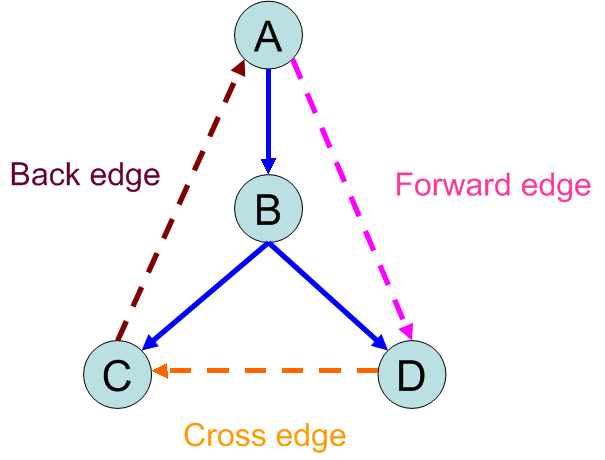
\includegraphics[width = 0.95\textwidth]{figs/dfs-digraph.png}
    \end{columns}
  \end{definition}

  \pause
  \vspace{0.50cm}
  \begin{itemize}
    \centering
    \item Also applicable to BFS
    \item w.r.t. DFS/BFS trees
  \end{itemize}
\end{frame}
%%%%%%%%%%%%%%%%%%%%

%%%%%%%%%%%%%%%%%%%%
\begin{frame}
  \begin{columns}
    \column{0.50\textwidth}
      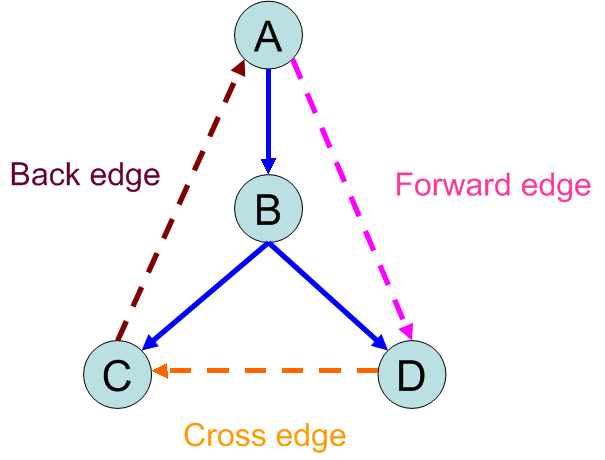
\includegraphics[width = 0.80\textwidth]{figs/dfs-digraph.png}

      \vspace{0.50cm}
      \centerline{\purple{DFS on directed graph}}
    \pause
    \column{0.50\textwidth}
      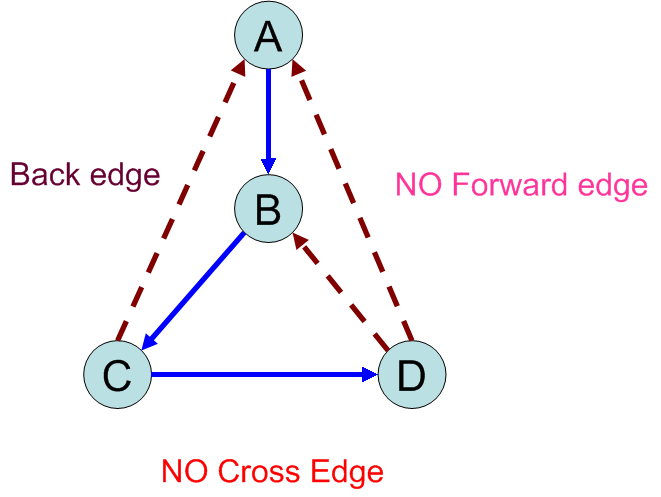
\includegraphics[width = 0.80\textwidth]{figs/dfs-undirected.png}

      \vspace{0.50cm}
      \centerline{\purple{DFS on undirected graph}}
  \end{columns}
\end{frame}
%%%%%%%%%%%%%%%%%%%%

%%%%%%%%%%%%%%%%%%%%
\begin{frame}
  \begin{columns}
    \column{0.50\textwidth}
      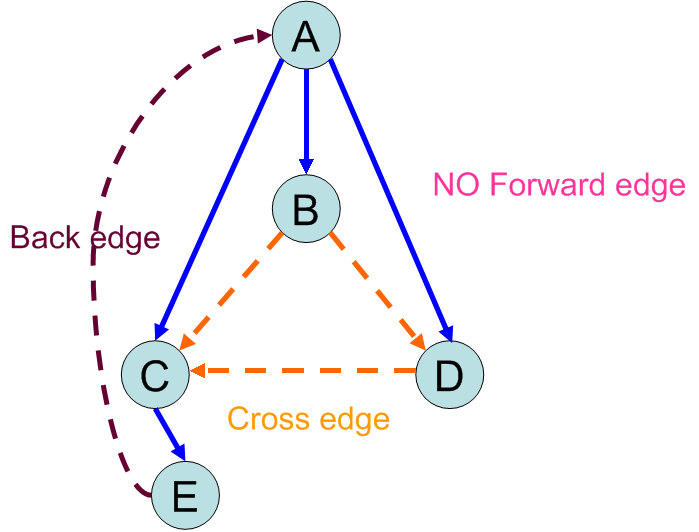
\includegraphics[width = 0.80\textwidth]{figs/bfs-digraph.png}

      \vspace{0.50cm}
      \centerline{\purple{BFS on directed graph}}
    \pause
    \column{0.50\textwidth}
      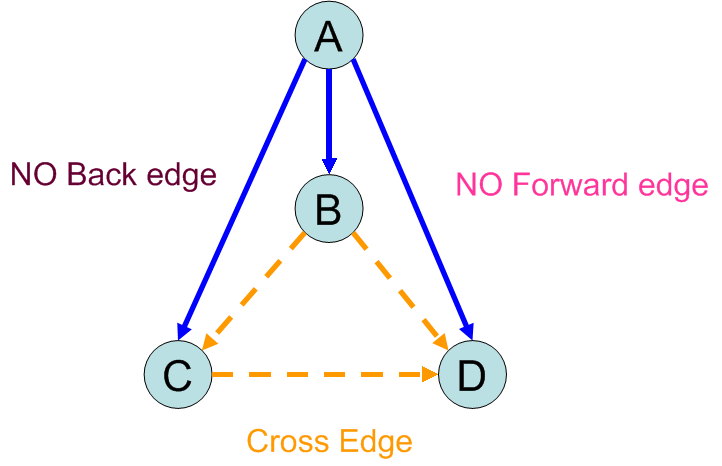
\includegraphics[width = 0.95\textwidth]{figs/bfs-undirected.png}

      \vspace{0.50cm}
      \centerline{\purple{BFS on undirected graph} \teal{\footnotesize (Problem $5.1$)}}
  \end{columns}
\end{frame}
%%%%%%%%%%%%%%%%%%%%

%%%%%%%%%%%%%%%%%%%%
\begin{frame}<presentation:0>[noframenumbering]
  \begin{exampleblock}{DFS tree and BFS tree coincide (Problem $5.7$)}
    \centerline{Undirected connected graph $G = (V,E), v \in V$}
      
    \[
      \text{DFS tree } T \text{ from } v \;\red{\equiv} \text{ BFS tree } T' \text{ from } v
    \]

    \pause
    \[
      \red{G \equiv T}
    \]
  \end{exampleblock}

  \pause
  \vspace{0.30cm}
  \begin{proof}
    \centerline{$G_{\text{DFS}}$: tree + back \emph{vs.} $G_{\text{BFS}}$: tree + cross}
  \end{proof}

  \pause
  \vspace{0.30cm}
  \begin{center}
    \red{$Q:$ What if $G$ is a digraph?}
  \end{center}
\end{frame}
%%%%%%%%%%%%%%%%%%%%
\begin{frame}{}
  \centerline{\red{\Large Life time of vertices in DFS}}
  \fig{width = 0.45\textwidth}{figs/active-interval.png}
\end{frame}
%%%%%%%%%%%%%%%%%%%%
\begin{frame}{}
  \begin{theorem}[Disjoint or Contained (Problem $4.2: (1) \& (2)$)]
    \[
      \forall u,v: [_{u} \; ]_{u} \cap [_{v} \; ]_{v} = \emptyset \bigvee 
      \Big([_{u} \; ]_{u} \subset [_{v} \; ]_{v} \lor [_{v} \; ]_{v} \subset [_{u} \; ]_{u}\Big)
    \]
  \end{theorem}

  \pause

  \begin{proof}
	\fig{width = 0.30\textwidth}{figs/stack.png}
  \end{proof}
\end{frame}
%%%%%%%%%%%%%%%%%%%%
\begin{frame}<presentation:0>[noframenumbering]
  \begin{exampleblock}{Preprocessing for \red{ancestor/descendant} relation (Problem $5.6$)}
    \fig{width = 0.42\textwidth}{figs/binary-tree}

    \centerline{\red{\large $Q:$ \it Is $u$ an ancestor of $v$? $O(1)$}}
  \end{exampleblock}

  \pause
  \[
    v: \text{d}[v], \text{f}[v]
  \]

  \pause
  \vspace{-0.20cm}
  \[
    \red{Q: } \text{ \# of descendants of any } v?
  \]
\end{frame}
%%%%%%%%%%%%%%%%%%%%

%%%%%%%%%%%%%%%%%%%%
\begin{frame}{}
  \begin{exampleblock}{Edge types and life time of vertices in DFS (Problem $4.5$)}
    \[
      \forall u \to v:
    \]
    \vspace{-0.30cm}
    \begin{itemize}
      \setlength{\itemsep}{5pt}
      \item tree/forward edge: $\red{[_{u}}\; \teal{[_{v}\; ]_{v}}\; \red{]_{u}}$
      \item back edge: $\teal{[_{v}}\; \red{[_{u}\; ]_{u}}\; \teal{]_{v}}$
      \item cross edge: $\teal{[_{v}\; ]_{v}}\; \red{[_{u}\; ]_{u}}$
    \end{itemize}
  \end{exampleblock}

  \pause
  \[
    \text{f}[v] < \text{d}[u] \iff \text{ \uncover<3->{\brown{cross}} edge}
  \]


  \[
    \uncover<4->{\text{f}[u] < \text{f}[v] \iff } \uncover<5->{\text{ \red{back} edge }}
  \]
  \[
    \uncover<6->{\nexists \text{ cycle} \implies \red{\boxed{u \to v \iff \text{f}[v] < \text{f}[u]}}}
  \]
\end{frame}
%%%%%%%%%%%%%%%%%%%%

%%%%%%%%%%%%%%%%%%%%
\begin{frame}<presentation:0>[noframenumbering]
  \centerline{\large DFS from the perspective of a single node:}
  
  \pause
  \fig{width = 0.30\textwidth}{figs/dfs-node-visiting}
\end{frame}
%%%%%%%%%%%%%%%%%%%%

%%%%%%%%%%%%%%%%%%%%
\begin{frame}<presentation:0>[noframenumbering]
  \begin{exampleblock}{Height and diameter of tree (Problem $5.4$)}
    Binary tree $T = (V, E)$ with $|V| = n$ and the root $r$:
    \begin{enumerate}[(I)]
      \item Height $H(T)$ in $O(n)$
      \item Diameter $D(T)$ in $O(n)$
    \end{enumerate}
  \end{exampleblock}

  \pause
  \vspace{0.20cm}
  \[
    \left\{\begin{array}{ll}
      \onslide<3->{H(T) = 0, & T \text{ is a leave} \\}
      H(T) = \max\Big(H(L_T), H(R_T)\Big) + 1, & \onslide<3->{\text{o.w.}}
    \end{array}\right.
  \]

  \pause
  \vspace{0.20cm}
  \onslide<4->{
    \[
      \left\{\begin{array}{ll}
	D(T) = 0, & T \text{ is a leave} \\
	\onslide<4->{D(T) = \max\Big(D(L_T), D(R_T), \onslide<5->{\underbrace{\red{H(L_T) + H(R_T) + 2}}_{\teal{\text{through the root}}}}\Big), & \text{o.w.}}
      \end{array}\right.
    \]
  }
\end{frame}
%%%%%%%%%%%%%%%%%%%%

%%%%%%%%%%%%%%%%%%%%
\begin{frame}<presentation:0>[noframenumbering]
  \centerline{Binary tree $T = (V, E)$ with $|V| = n$ and the root $r$}

  \pause
  \vspace{0.80cm}
  \centerline{\red{$Q:$ Diameter of a \blue{\it tree} \teal{\it without} a designated root}}

  \pause
  \fig{width = 0.40\textwidth}{figs/tree-no-root}
\end{frame}
%%%%%%%%%%%%%%%%%%%%

%%%%%%%%%%%%%%%%%%%%
\begin{frame}<presentation:0>[noframenumbering]
  \centerline{\red{$Q:$ Diameter of a tree \teal{\it without} a designated root}}

  \pause
  \vspace{0.80cm}
  \begin{columns}
    \column{0.60\textwidth}
      {\large A beautiful algorithm:}
      \begin{itemize}
	\item Pick any $u$
	\item Run BFS from $u$, obtain the farthest $v$
	\item Run BFS from $v$, obtain the farthest $w$
      \end{itemize}
      \[
	(v, w)
      \]
    \pause
    \column{0.20\textwidth}
      \centerline{\red{\blue{Your Job:} Prove it!}}
  \end{columns}

  \pause
  \vspace{0.50cm}
  \centerline{\teal{Back to our original problem with $u \gets r$.}}
\end{frame}
%%%%%%%%%%%%%%%%%%%%

%%%%%%%%%%%%%%%%%%%%
\begin{frame}<presentation:0>[noframenumbering]
  \begin{exampleblock}{Perfect subtree (Problem $5.5$)}
    \begin{itemize}
      \item binary tree $T = (V, E)$
      \item root $r \in V$
      \item goal: find all perfect subtrees
    \end{itemize}
  \end{exampleblock}
\end{frame}
%%%%%%%%%%%%%%%%%%%%

%%%%%%%%%%%%%%%%%%%%
\begin{frame}{}
  \begin{exampleblock}{Counting shortest paths (Problem $5.10$)}
    Counting \# of shortest paths in (un)directed graphs using BFS.
  \end{exampleblock}

  \pause
  \vspace{0.50cm}
  \centerline{Maybe in the next class$\dots$}
\end{frame}
%%%%%%%%%%%%%%%%%%%%
